\begin{definition}{Réseaux de décisions}{decisionnet}
    Un réseau de décision, également connu sous le nom de réseau de décision bayésien (RDB), 
    est un modèle graphique probabiliste qui étend le concept de réseau bayésien pour inclure la prise 
    de décision dans un environnement incertain. Un réseau de décision intègre des éléments tels que des 
    actions et des utilités pour modéliser des situations où des décisions doivent être prises dans un contexte de probabilités et d'incertitude.
    Il est composé de trois types de nœuds : les nœuds de décision, les nœuds de chance et les nœuds d'utilité. 
    \begin{itemize}
        \item \textbf{Nœuds de décision} : Les nœuds de décision sont des nœuds carrés qui représentent les actions à prendre. 
        \item \textbf{Nœuds de chance} : Les nœuds de chance sont des nœuds ovales qui représentent les événements incertains. Comme dans les réseaux bayésiens.
        \item \textbf{Nœuds d'utilité} : Les nœuds d'utilité sont des nœuds hexagonaux qui représentent les fonctions d'utilité. Il est souvent fils d'un nœud de décision et/ou d'un nœud de chance.
    \end{itemize}
    Son but est de trouver la meilleure action.
\end{definition}

Voici l'algorithme pour trouver la meilleure action.

\begin{itemize}[label=\textbullet]
    \item Instancier les nœuds de chance avec les valeurs observées (n'import laquelle). Instancier les observations.
    \item Pour chaque action
        \begin{itemize}[label=\textbullet]
            \item Instancier action par une valeure. (celle qui nous intéresse).
            \item Pour chaque noeuds d'utilité, calculer la probabilité à postériori de ses parents selon les observations.
            \item Pour chaque noeuds d'utilité, calculer la valeur de l'utilité attendue.
        \end{itemize}
    \item Choisir l'action qui maximise l'utilité attendue.
\end{itemize}

\begin{example}\leavevmode
    \begin{figure}[H]
        \centering
        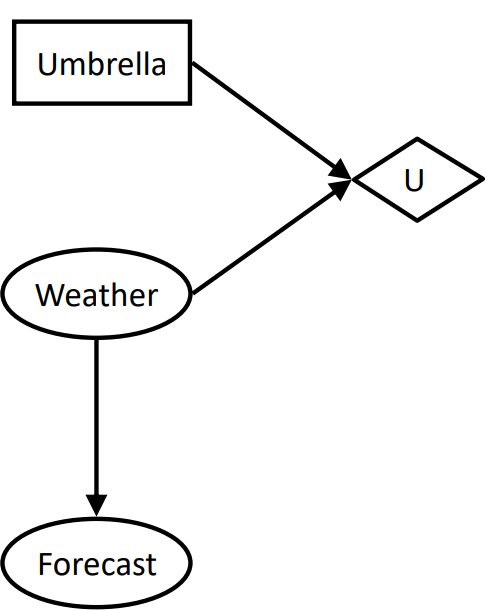
\includegraphics[width=0.3\textwidth]{pictures/decisonnet.png}
        \caption{Réseau de décision}\label{fig:decisionnet}
    \end{figure}

    Umbrella est l'action de prendre, ou non, un parapluie. Il y a deux nœuds de chance : le premier $Weather$
    est le nœud de chance de la météo, qui peut être soit pluvieux, soit ensoleillé. 
    Le second, $Forecast$, est le nœud de chance de la prévision météorologique, qui peut être soit pluvieux, soit ensoleillé.
    Il y a un nœud d'utilité, $U$, qui représente le coût de prendre un parapluie.

    Pour calculer la probabilité à postériori de $Weather$, $P(W | e, a)$.

    Pour calculer l'utilité attendue, $EU(a) = \sum_{w} P(w | e, a) U(w, a)$. Car en effet,
    $U$ dépend de $Weather$ et de $Umbrella$.
\end{example}

Nous pouvons représenter un réseau de décision par un arbre de "résultat" (outcome tree). Ces même arbres 
sont utilisé pour représenter l'algorithme \textbf{Expectimax}.
Sauf que cette fois pour avoir la probabilités des noeuds de chance, il faut calculer la probabilité à postériori dans un réseau bayésien.

\begin{figure}[H]
    \begin{center}
        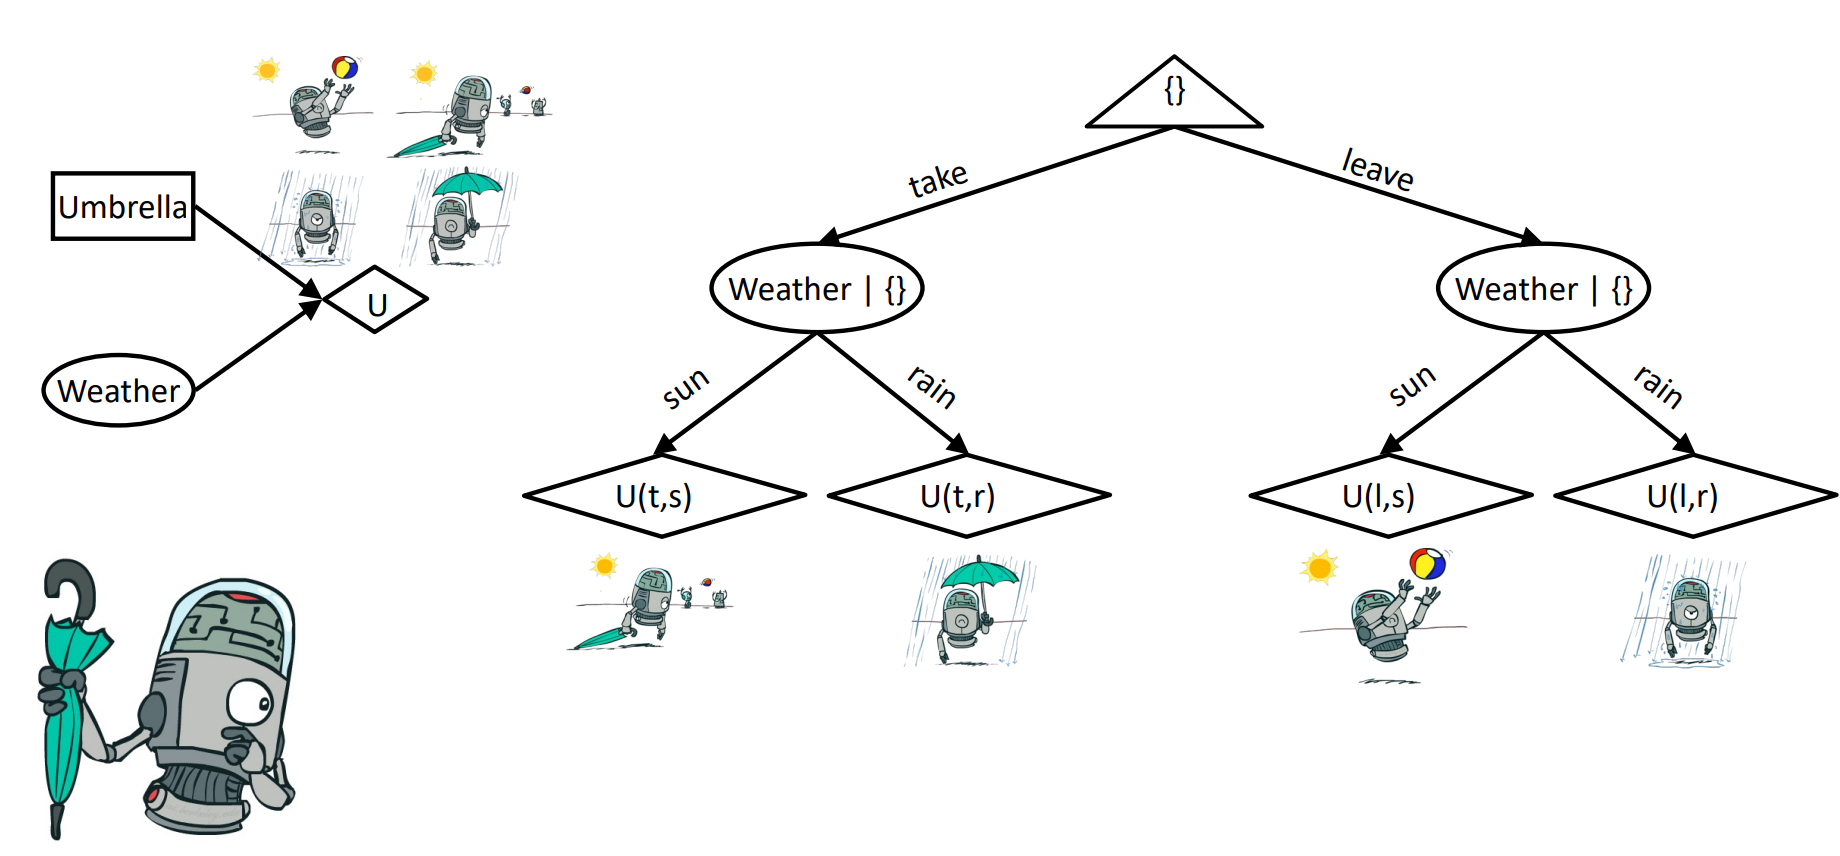
\includegraphics[width=0.5\textwidth]{pictures/decisionnetasoutcometree.png}
    \end{center}
    \caption{Arbre de résultat}\label{fig:decisionnetasoutcometree}
\end{figure}

\subsection{Value of Perfect Information} % (fold)
\label{sub:value_of_perfect_information}

\begin{definition}{Value of Perfect Information}{valueofperfectinformation}
    La valeur de l'information parfaite est la différence entre l'utilité attendue maximale avec l'information parfaite et l'utilité attendue maximale sans l'information parfaite.
    \begin{equation}
        VPI = EU_{max}^{PI} - EU_{max}^{NPI}
    \end{equation} 
    où $PI$ est l'information parfaite et $NPI$ est sans l'information parfaite.
\end{definition} 

\begin{remark}\leavevmode
    De ce que j'ai compris, l'information parfaite correspond à la révélation d'un noeud de chance dans le réseau de décision.
\end{remark}

Imaginons que nous avons les observations $E = e$. Pour calculer l'utilité on a: 
\begin{equation*}
    MEU(e) = \max_{a} \sum_{w} P(s | e) U(s, a)
\end{equation*}
où $s$ est l'état du monde.

Si on apprend qu'il existe une information $E'=e'$ qui est rend plus précis notre calcul de l'utilité, on a: 
\begin{equation*}
    MEU(e, e') = \max_{a} \sum_{w} P(s | e, e') U(s, a) 
\end{equation*}
Cependant, on n'a pas cette information. Celle-ci est aussi incertaine. Il faut donc calculer la distribution de probabilité de $E'$. 
\begin{equation*}
    MEU(e, E') = \sum_{e'} P(e'|e) MEU(e, e')
\end{equation*}

Le \textbf{VPI} est donc l'information de combien l'utilité attendue augmente si on a l'information $E'$ qui nous est révélée.
\begin{equation*}
    VPI = MEU(e, E') - MEU(e)
\end{equation*}


Voici les propriétés du \textbf{VPI}: 
\begin{itemize}[label=\textbullet]
    \item $VPI \geq 0$ 
    \item $VPI$ est non-additif. $VPI(E_1, E_2| e) \neq VPI(E_1| e) + VPI(E_2| e)$
    \item $VPI$ Ne dépend pas de l'ordre dans lequel les informations sont révélées. $VPI(E_1, E_2| e) = VPI(E_2, E_1| e)$

\end{itemize}

Si il y a une observation $Z$ qui est conditionnellement indépendante à $Parent(U)$ sachant les autres observations ALORS 
le \textbf{VPI} est égal à $0$.



% subsection Value of Perfect Information (end)


